\apendice{Documentación de usuario}
\section{Introducción}
Llegados al fin del proyecto quedaría como resultado para el usuario, una aplicación software que desde Unity con unas gafas como las Oculus Quest 2 se nos permita hacer uso de un robot mediante teleoperación. 
\section{Requisitos de usuarios}
Para poder hacer uso del software desarrollado necesitamos fundamentalmente dos dispositivos hardware relacionados con la realidad virtual distintos que son las Oculus Quest 2 y los Nova de SenseGlove, un robot con ROS como el Kinova 6DOF y un ordenador con Unity.
Para poder instalar y ejecutar correctamente Unity los requisitos son los mismos que los expuestos previamente:
\begin{figure}[h]
\centering
\label{Requisitos minimos y recomendados Unity}
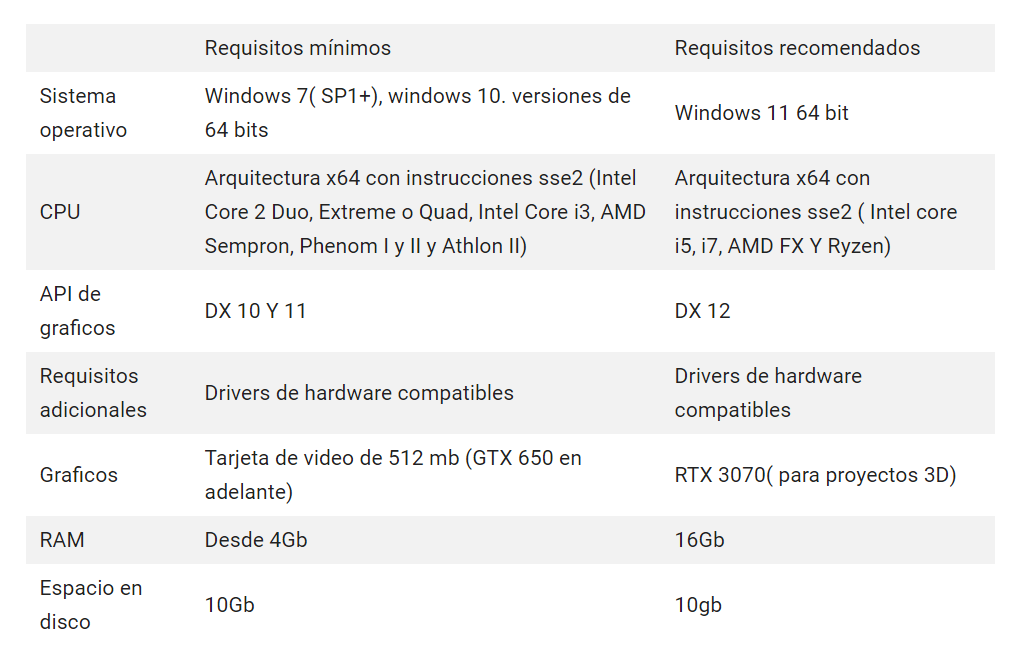
\includegraphics[width=\textwidth]{img/unity req.PNG}
\caption{Requisitos minimos y recomendados Unity}
\end{figure}

\newpage
\section{Instalación}

En cuanto a los pasos para completar la instalación del proyecto en el ordenador de un usuario, son los mismos que los expuestos en el previo apartado de \textit{Compilación, instalación y ejecución del proyecto}

\section{Manual del usuario}
Tras la debida preparación en apartados anteriores de nuestos dispositivos, una vez tengamos todos calibrados y con conexión con el PC o el robot, lo único que tenemos que hacer es ejecutar el software y aplicar sobre nuestra mano los debidos desplazamientos deseados para mover la pinza o gestualizar el cierre de la misma para controlar su apertura.

